\section{Rotating Frame of Reference}
\subsection{Little problem}
When a person is standing (on Earth) there are two forces acting on them:\\

\columnratio{0.4, 0.6}
\begin{paracol}{2}
    \begin{leftcolumn}
        \begin{figure} \label{fig:2.1}
        \centering
            \includegraphics[width=0.2\textwidth]{pictures/FBD2.6.1.png}
        \caption{Normal force and Gravity}
        \end{figure}
        
    \end{leftcolumn}

    \begin{rightcolumn}
        The normal force acting on the person is pushing force, thus a force of \textbf{compresion}. An object 
        that has a compression force must be able to \textbf{withstand this force} or it will collapse. (See \ref{fig:2.1})\\

        In the caes of a person, their muscles and their bones must be able to withstand this force, thus you 
        \textbf{muskule-skeletal system develops} to withstand this force
    \end{rightcolumn}
\end{paracol}

When a person is in orbit around a planet, there is only the force of gravity acting on them! They are in 
\textbf{constant state of free fall} \\

FBD for a person orbiting a planet:
\columnratio{0.4, 0.6}
\begin{paracol}{2}
    \begin{leftcolumn}
        \begin{figure}
            \centering
            \includegraphics[width=0.2\textwidth]{pictures/FBD2.png}
            \caption{Force of Gravity}
        \end{figure}
    \end{leftcolumn}
    \begin{rightcolumn}
        The person is missing the \textbf{normal force} (the compressive force) that they are used to feeling. 
        Without the compressive force, the person's musculo=skeletal system starts to undergo \textbf{atrophication}
    \end{rightcolumn}
\end{paracol}

To solve this problem, we need to make sure that both two forces are acting on the person. The forces must 
be in \textbf{opposite direction} and one force must be a \textbf{compression force}\\

\subsection*{Solution 1}
The spaceship is \textbf{accelerating} uniformly, in a straight line.\\

But, there are two problems:
\begin{enumerate}
    \item Run out of fuel
    \item As an object speed up, its \textbf{mass increases}. If mass increases, to maintain the acceleration the netforce would also increase
\end{enumerate}

\subsection*{Solution 2}
Get a very very large hallow ring and make it spin\\

For an internal F.O.R, there will be both \textbf{Force of Normal} and \textbf{Force of Gravity} acting on it\\

From an internal F.O.R:
\begin{gather*}
    \sum \vec{F} = m \vec{a_{per}}\\
    F_{N} - F_{fict} = 0\\
    F_{N} = F_{fict}\\
    F_{N} = m*\left| a_{F.O.R}\right| \\
    F_{N} = ma_{c}
\end{gather*}

We can calculate the $v$ of the people:
\begin{gather*} 
    F_{N} = ma_{c}\\
    mg = ma_{c}\\
    g = a_{c}\\
    g = \frac{v^2}{R}\\
    v = \sqrt{gR}
\end{gather*}

So, in the spaceship rotating question, we can always assume:
\begin{equation*}
    F_{N} = F_{g}
\end{equation*}

We can also using
\begin{equation*}
    a_{c} = \frac{4 \pi^2 R}{T^2}
\end{equation*}

To sub in
\begin{gather*}
    g = \frac{4 \pi^2 R}{T^2}\\
    T = \sqrt{\frac{4 \pi^2 R}{g}}
\end{gather*}
or
\begin{equation*}
    f = \sqrt{\frac{g}{4 \pi^2 R}}
\end{equation*}

\subsection{Perceived Acceleration in a Rotating Frame of Reference}
When a person is stand on the equator, there are $a_{c}$ to affect the ball\\

The \textbf{perceived} acceleration should be calculated like this:

\begin{center}
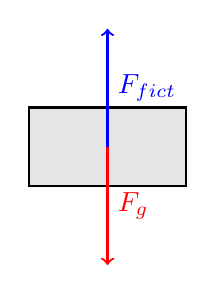
\begin{tikzpicture}[scale=1]
    % Draw the block
    \draw[thick, fill=gray!20] (0,0) rectangle (2,1);
    
    % Draw the surface
    % \draw[thick] (-1,0) -- (3,0);
    
    % Draw the forces
    % Gravity
    \draw[->, thick, red] (1,0.5) -- (1, -1) node[midway, right] {$F_g$};
    % Normal
    \draw[->, thick, blue] (1,0.5) -- (1, 2) node[midway, right] {$F_{fict}$};
    % Friction
    % \draw[->, thick, green] (1,0.5) -- (-1, 0.5) node[midway, above] {$F_f$};
\end{tikzpicture}
\end{center}

Now, let's calculate the $\vec{a_{per}}$
\begin{gather}
    \sum \vec{F} = m\vec{a_{per}}\\
    F_N - F_{fict} = ma_{per}\\
    mg - m\left|a_{F.O.R}\right| = ma_{per}\\
    a_{per} = g - a_c
\end{gather}

\subsection*{Note}
    You can always assume Earth's surface to be an inertial F.O.R unless:
    \begin{itemize}
        \item You need to be \textbf{extremely accurate}
        \item The question states \textbf{at the equator}
    \end{itemize}